\section{Rundenfunktion}
\label{sec:sha256:runde}

Die Rundenfunktion ist in Abbildung \ref{fig:sha256core} dargestellt und ähnelt der eines doppelten Feistel-Netzwerks.
Es kommen sowohl die modulare 32-Bit Addition, die Choose- und Majority-Funktion, wie auch die beiden $\Sigma$-Funktionen zum Einsatz.
Bei einem Feistel-Netzwerk wird im allgemeinen ein Teil der Eingabe direkt in die Ausgabe kopiert während der andere
Teil unter Verwendung des ersten Teils verschlüsselt wird \cite[311]{crypto1}. Direkt kopiert werden sowohl A bis C
als auch E bis G. A' wird mit Hilfe von A bis C berechnet, während E' mit Hilfe von E bis G berechnet wird.
Als Schlüssel fließen D, H und I mit ein.

Initialisiert werden A bis H in der ersten Runde der ersten Kompression mit 8 Konstanten. Für die Konstanten mit 32 Bit Breite wurden laut
Standard \cite[10]{nist1804} die Quadratwurzel der ersten 8 Primzahlen herangezogen. Die ersten 32 Bit der Dezimalstellen jeder Quadratwurzel
ergeben die jeweilige Konstante. Mit Blick auf das Feistel-Netzwerk lassen sich diese Konstanten mit dem Klartext vergleichen, der mit der
Eingabe als Schlüssel zum Geheimtext entwickelt wird.

Enthalten ist in Abbildung \ref{fig:sha256core} auch die Addition der Rundenkonstante (K+). Für die Rundenkonstanten wurden laut Standard
\cite[10]{nist1804} die Kubikwurzel der ersten 64 Primzahlen herangezogen. Die ersten 32 Bit der Dezimalstellen jeder Kubikwurzel ergeben
die jeweilige Konstante. Die Addition der Konstanten bewirkt, dass der Einfluss der Eingabe sich in jeder Runde unterschiedlich auswirkt.

\begin{figure}[!h]
  \centering
  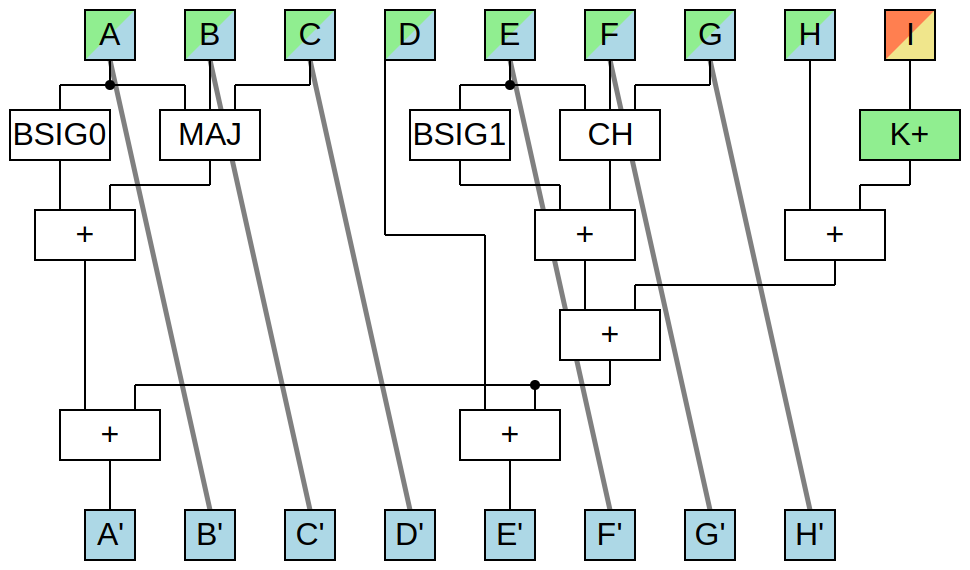
\includegraphics[scale=0.4]{images/sha256core}
  \caption{Schematische Darstellung einer SHA256-Runde}
  \label{fig:sha256core}
\end{figure}